\documentclass[aspectratio=169, pdf, 8pt, unicode]{beamer}
\usepackage[american,russian]{babel}
\usepackage[default]{sourcesanspro}
\usepackage{float}
\usepackage{graphicx}
\usepackage{pgfplotstable}
\usepackage{caption}
\usepackage{amsmath}
\usepackage{amssymb}
\usepackage{setspace}
\usepackage{fancyvrb}
\usepackage[outputdir=aux]{minted}

\DeclareCaptionLabelFormat{gostfigure}{Рисунок #2}
\captionsetup[table]{labelsep=endash,justification=justified,singlelinecheck=false,font=normalsize,skip=0pt} 
\captionsetup[figure]{labelformat=gostfigure,labelsep=endash,justification=centering,singlelinecheck=false,font=normalsize} 
\pgfplotsset{compat=1.9}

\mode<presentation> {
\usetheme{Madrid}
}

\setbeamerfont{institute}{size=\normalsize}
\setbeamertemplate{itemize/enumerate body begin}{\large}
\setbeamertemplate{itemize/enumerate subbody begin}{\tiny}

\title[Теория и практика многопоточного программирования]{Теория и практика многопоточного программирования}

\author{Неганов Алексей}

\institute[МФТИ]{
    Московский физико-технический институт (национальный исследовательский университет)\\
    Кафедра теоретической и прикладной информатики\\
}

\date{Москва 2020}

\setbeamertemplate{caption}[numbered]

\begin{document}

\begin{frame}
\titlepage
\end{frame}

\begin{frame}[fragile]
\frametitle{RMW-операции: ABA}

\begin{minipage}{0.4\textwidth}
\begin{small}
\begin{verbatim}
 1 struct node {
 2       struct node *next;
 3 }
 4
 5 static struct node *top = NULL;
 6 
 7 void push(struct node *n) {
 8       do {
 9             struct node *t = top;
10             n->next = t;
11       } while (!CAS(&top, t, n));
12 }
13
14 void struct node *pop(void) {
15       struct node *next;
16       do {
17             struct node *t = top;
18             if (t == NULL)
19                   return NULL;
20             next = t->next;
21       } while (!CAS(&top,t,next));
22       return t;
23 }
\end{verbatim}
\end{small}
\end{minipage}%
\begin{minipage}{0.4\textwidth}
\begin{small}
\begin{verbatim}
Thread #1:                     Thread #2:

struct node *a = pop();        struct node *b = pop();
                               pop();
                               push(b);
\end{verbatim}
\end{small}
\end{minipage}%
\end{frame}

\begin{frame}[fragile]
\frametitle{Tagged pointers}
\begin{figure}[H]
\centering
\begin{minipage}{0.8\textwidth}
\begin{verbatim}
// linux/include/linux/rbtree.h

struct rb_node {
    unsigned long  __rb_parent_color;
    struct rb_node *rb_right;
    struct rb_node *rb_left;
} __attribute__((aligned(sizeof(long))));

#define rb_parent(r)   ((struct rb_node *)((r)->__rb_parent_color & ~3))
\end{verbatim}
\end{minipage}%
\caption{Простой пример использования свободных бит в указателе}
\end{figure}
\end{frame}

\begin{frame}[fragile]
\frametitle{Tagged pointers}
\begin{figure}[H]
\centering
\begin{minipage}{0.8\textwidth}
\small
\begin{verbatim}
// boost/lockfree/detail/tagged_ptr_ptrcompression.hpp

template <class T>
class tagged_ptr
{
    typedef boost::uint64_t compressed_ptr_t;
public:
    typedef boost::uint16_t tag_t;
private:
    union cast_unit {
        compressed_ptr_t value;
        tag_t tag[4];
    };
    static const int tag_index = 3;
    static const compressed_ptr_t ptr_mask = 0xffffffffffffUL; //(1L<<48L)-1;
    static T* extract_ptr(volatile compressed_ptr_t const & i) {
        return (T*)(i & ptr_mask);
    }
    static tag_t extract_tag(volatile compressed_ptr_t const & i) {
        cast_unit cu;
        cu.value = i;
        return cu.tag[tag_index];
    }
\end{verbatim}
\end{minipage}%
\caption{Пример использования старших 16 бит}
\end{figure}
\end{frame}

\begin{frame}[fragile]
\frametitle{Tagged pointers: пример использования}
\begin{figure}[H]
\centering
\begin{minipage}{0.8\textwidth}
\small
\begin{verbatim}
template <typename T> struct node {
    tagged_ptr next;
    T data;
} ;

template <typename T> class MSQueue {
   tagged_ptr<T> volatile m_Head;
   tagged_ptr<T> volatile m_Tail;

   FreeList m_FreeList;
public:
   MSQueue() {
     m_Head.ptr = m_Tail.ptr = new node();
   }
};
\end{verbatim}
\end{minipage}%
\end{figure}
\end{frame}

\begin{frame}[fragile]
\frametitle{Tagged pointers: пример использования}
\begin{figure}[H]
\centering
\begin{minipage}{0.8\textwidth}
\small
\begin{verbatim}
void enqueue( T const& value ) {
E1: node * pNode = m_FreeList.newNode();
E2: pNode–>data = value;
E3: pNode–>next.ptr = nullptr;
E4: for (;;) {
E5:   tagged_ptr<T> tail = m_Tail;
E6:   tagged_ptr<T> next = tail.ptr–>next;
E7:   if tail == m_Tail {
E8:      if next.ptr == nullptr {
E9:         if CAS(&tail.ptr–>next, next, tagged_ptr<T>(node, next.tag+1)) {
E10:          break; // success!
            }
E11:     } else {
E12:        CAS(&m_Tail, tail, tagged_ptr<T>(next.ptr, tail.tag+1)); // tail is not the last
         }
      }
    } // end loop
E13: CAS(&m_Tail, tail, tagged_ptr<T>(pNode, tail.tag+1)); // tail to inserted
}
\end{verbatim}
\end{minipage}%
\end{figure}
\end{frame}

\begin{frame}[fragile]
\frametitle{Tagged pointers: пример использования}
\begin{figure}[H]
\centering
\begin{minipage}{0.8\textwidth}
\small
\begin{verbatim}
bool dequeue( T& dest ) {
D1:  for (;;) {
D2:    tagged_ptr<T> head = m_Head;
D3:    tagged_ptr<T> tail = m_Tail;
D4:    tagged_ptr<T> next = head–>next;
D5:    if ( head == m_Head ) {
D6:       if ( head.ptr == tail.ptr ) {
D7:         if (next.ptr == nullptr )
D8:              return false; // queue is empty
D9:         CAS(&m_Tail, tail, tagged_ptr<T>(next.ptr, tail.tag+1>)); // tail to last
D10:      } else {
D11:        dest = next.ptr–>data;
D12:        if (CAS(&m_Head, head, tagged_ptr<T>(next.ptr, head.tag+1))
D13:           break // success
          }
       }
     } // end of loop
D14: m_FreeList.add(head.ptr);
D15: return true;
}
\end{verbatim}
\end{minipage}%
\end{figure}
\end{frame}

\begin{frame}[fragile]
\frametitle{Epoch-based reclamation}
\begin{figure}[H]
\centering
\begin{minipage}{0.8\textwidth}
\small
\begin{verbatim}
static atomic<unsigned int> m_nGlobalEpoch := 1 ;

const EPOCH_COUNT = 3 ;

struct ThreadEpoch {
    unsigned int m_nThreadEpoch ;
    // deferred for reclamation
    List<void *> m_arrRetired[ EPOCH_COUNT ] ;

    ThreadEpoch(): m_nThreadEpoch(1) {}

    void enter() {
       if ( m_nThreadEpoch <= m_nGlobalEpoch )
          m_nThreadEpoch = m_nGlobalEpoch + 1 ;
    }

    void exit() {
       if ( each thread epoch is greater than m_nGlobalEpoch ) {
          ++m_nGlobalEpoch ;

          // for each thread free elements
          m_arrRetired[ (m_nGlobalEpoch – 1) % EPOCH_COUNT ]
       }
    }
} ;
\end{verbatim}
\end{minipage}%
\end{figure}
\end{frame}

\begin{frame}[fragile]
\frametitle{Hazard pointers}
\begin{figure}
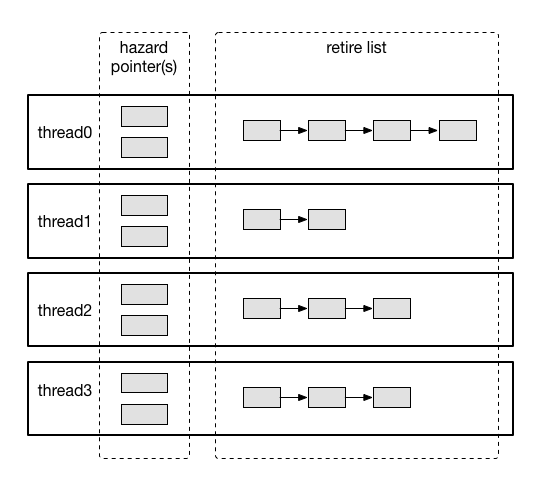
\includegraphics[width=0.5\textwidth]{fig/hp.png}
\end{figure}
\texttt{https://github.com/concurrencykit/ck/blob/master/src/ck\_hp.c}
\end{frame}

\begin{frame}[fragile]
\frametitle{Hazard pointers}
\begin{figure}[H]
\centering
\begin{minipage}{0.45\textwidth}
\small
\begin{verbatim}

// per-thread HP array
// only owner can write, everybody can read
void *HP[HP_NUM]; 

unsigned dcount = 0; // dlist used
void* dlist[BATCH_SIZE]; // to delete

void RetireNode(void *node) { 
  dlist[dcount++] = node;
  if (dcount == BATCH_SIZE)
     Scan();
}

void Scan() { 
   unsigned p=0;
   void * plist[HP_NUM*THR_NUM];

   // Stage 1: collect all HPs
   for (unsigned t=0; t < THR_NUM; ++t) {
      void **pHPThread = get_thread_data(t)->HP;
      for (unsigned i = 0; i < HP_NUM; ++i) {
         void *hptr = pHPThread[i];
         if ( hptr != nullptr )
            plist[p++] = hptr;
      }
   }

\end{verbatim}
\end{minipage}%
\hspace{0.5mm}
\begin{minipage}{0.45\textwidth}
\small
\begin{verbatim}
   // Stage 2: sort HPs (prepare the search)
   sort(plist);

   // Stage 3: delete all non-hazard items
   unsigned new_dcount = 0;
   void *new_dlist[HP_NUM*THR_NUM];
   for ( i = 0; i < BATCH_SIZE; ++i ) {
      if ( binary_search(dlist[i], plist))
         new_dlist[new_dcount++] = dlist[i];
      else
         free(dlist[i]); // non-hazard
   }

   // Stage 4: reinitialize dlist
   for (i = 0; i < new_dcount; ++i ) 
      dlist[i] = new_dlist[i]; 
   dcount = new_dcount;
}
\end{verbatim}
\end{minipage}%
\end{figure}
\end{frame}

\begin{frame}[fragile]
\frametitle{RCU}
\begin{figure}[H]
\centering
\begin{minipage}{0.8\textwidth}
\small
\begin{verbatim}
rcu_read_lock( ... );
stuff = find_the_stuff(args);
do_something_with(args);
rcu_read_unlock();
\end{verbatim}
\end{minipage}%
\end{figure}
\begin{figure}
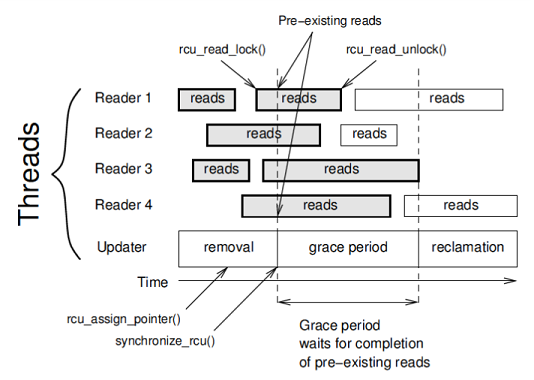
\includegraphics[width=0.5\textwidth]{fig/rcu.png}
\end{figure}
\end{frame}

\begin{frame}[fragile]
\frametitle{RCU}
\begin{figure}[H]
\centering
\begin{minipage}{0.8\textwidth}
\small
\begin{verbatim}
void rcu_read_lock(void) {}

void rcu_read_unlock(void) {}

void call_rcu(void (*callback) (void *), void *arg) {
    // add callback/arg pair to a list
}

void synchronize_rcu(void) {
    int cpu, ncpus = 0;

    for_each_cpu(cpu)
        schedule_current_task_to(cpu);

        for each entry in the call_rcu list
            entry->callback (entry->arg);
}
\end{verbatim}
\end{minipage}%
\end{figure}
\end{frame}

\begin{frame}[fragile]
\frametitle{User-space RCU}
\begin{itemize}
\item Quiescent-State-Based Reclamation RCU
\item General-Purpose URCU
\item RCU via Signal Handling
\end{itemize}
\end{frame}

\end{document}
